
\فصل{ارزیابی روش پیشنهادی}

در این فصل به ارزیابی روش پیشنهادی و مقایسه‌ی آن با چهار روش پی.اِم، دوچی، رپور و دی.بیت.فلیپ.پی.اِم می‌پردازیم. معیارهای خطای مجذور میانگین و اختلاف احتمال توزیع داده‌ها برای داده‌های با ابعاد بالا (روش‌های پی.اِم و دوچی) در نظر گرفته شده است. همچنین تخمین شمارش داده‌ها در مقایسه با پژوهش‌های مربوط به داده‌های در حال تغییر (روش‌های رپور و دی.بیت.فلیپ.پی.اِم) بررسی می‌شود. 

در این بخش ابتدا مجموعه داده ورودی معرفی شده و سپس نتایج ارزیابی روی دو دسته‌ی مذکور از داده‌ها بیان می‌شود. لازم به ذکر است که روش پیشنهادی همواره روی مجموعه‌ای از داده‌ها اجرا شده است که هم دارای ابعاد بالا بوده و هم به صورت مکرر تغییر می‌کنند. نتایج نشان می‌دهد که روش پیشنهادی با حفظ حریم خصوصی تفاضلی محلی، کارایی بهتری نسبت به الگوریتم‌های پیشین دارد.

\قسمت{مجموعه داده‌ی ورودی}

 به منظور ارزیابی راهکار پیشنهادی از مجموعه داده‌ی بزرگسالان\پانویس{Adult} استفاده شده است. این پایگاه داده از سرشماری سال ۱۹۹۴ ایالات متحده استخراج شده و یکی از معروف‌ترین مجموعه داده‌ها در حوزه یادگیری ماشین برای کارهای طبقه‌بندی است.

داده‌ها از نوع اعداد صحیح بوده و شامل اطلاعات شخصی و جمعیت‌شناختی افراد است. در این مجموعه داده ویژگی‌هایی مانند سن، سطح تحصیلات، وضعیت تاهل، نژاد و جنسیت وجود دارد. 15 ویژگی و 45222 رکورد از کاربران در این مجموعه داده گنجاده شده است و برای تست عملکرد الگوریتم روی داده‌های غیر دودویی و عددی که دارای همبستگی‌های پیچیده بین ویژگی‌های مختلف هستند، بسیار مفید است.

به منظور ارزیابی عملکرد راهکار پیشنهادی روی داده‌های در حال تغییر، از مجموعه‌ داده‌ی گردآوری شده در پژوهش لولوها استفاده شده است. نویسندگان این پژوهش یک مجموعه داده‌ی مصنوعی به اسم «سین\پانویس{Syn}» تهیه کرده اند. این مجموعه داده برای شبیه‌سازی دنیای واقعی طراحی شده است که در آن، داده‌ها به صورت دوره‌ای و مکرر (هر 6 ساعت یکبار) جمع‌آوری شده اند.

اندازه دامنه ۳۶۰ است که در واقع همان تعداد دقایق در یک بازه ۶ ساعته است. مجموعه داده سین از 10000 کاربر به تعداد 120 بار جمع‌آوری شده است. نحوه ساخت این داده‌ها طوری است که به خوبی وضعیت داده‌های در حال تغییر را شبیه سازی می‌کند.

به منظور ساخت مجموعه داده‌ای که هر دو ویژگی مطرح را داشته باشد باید دو مجموعه داده‌ی ذکر شده را با یکدیگر ترکیب کنیم. مطابق شکل \رجوع{fig:dataset} مجموع داده‌ی سین به صورت یک بُعد در کنار 15 بُعد مجموعه داده بزرگسالان قرار می‌گیرد.

\begin{figure}[h]
  \centering
  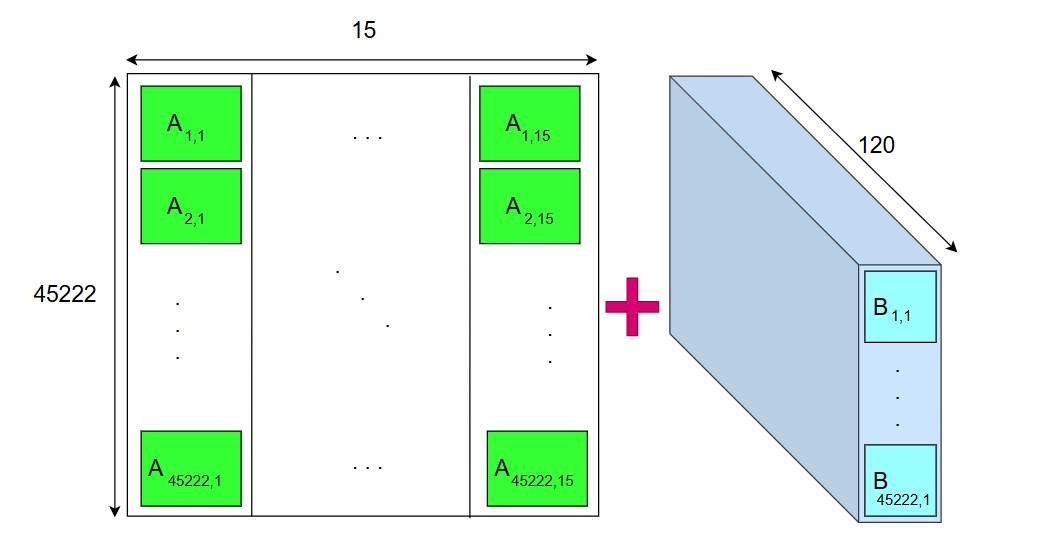
\includegraphics[width=0.9\textwidth]{figs/dataset.jpg}
  \caption{نحوه ترکیب دو مجموعه داده‌ی بزرگسالان و سین. مشخصه‌ی $A_{i,j}$ نشان دهنده‌ی ویژگی $j$ام از کاربر $i$ام است. همچنین نشان $B_{i,t}$، داده‌ی پویای کاربر $i$ام در واحد زمانی $t$ام را نمایش می‌دهد.}
  \label{fig:dataset}
\end{figure}

\قسمت{ارزیابی روی داده‌های با ابعاد بالا}

در این بخش معیار میانگین مربعات خطا و میانگین اختلاف توزیع احتمال داده‌ها با دو روش پی.اِم و دوچی مقایسه می‌شود.

\زیرقسمت{ارزیابی حین تغییر بودجه‌ی حریم خصوصی}

نمودار \رجوع{fig:eps_mse}، میانگین مربعات خطا را برای سه روش مختلف حفظ حریم خصوصی در برابر بودجه‌ی حریم خصوصی مقایسه می‌کند. محور عمودی نشان‌دهنده خطای روش و محور افقی، میزان بودجه حریم خصوصی است؛ هرچه $\epsilon$ بزرگ‌تر باشد، سطح حریم خصوصی کمتر و دقت مورد انتظار بالاتر است.

همانطور که در نمودار مشخص است، روش پیشنهادی (خط آبی) در تمام نقاط، به طور مداوم کمترین میزان خطا را نسبت به دو روش دیگر، یعنی روش پی.اِم و روش دوچی، به ثبت رسانده است. این موضوع بیانگر عملکرد برتر و دقت بالاتر الگوریتم ارائه‌شده است. روش دوچی در مقادیر پایین $\epsilon$، خطای بسیار بالایی دارد که با افزایش $\epsilon$ به سرعت کاهش می‌یابد اما همچنان بالاتر از دو روش دیگر باقی می‌ماند. روش پی.اِم عملکرد بهتری نسبت به روش دوچی دارد اما کماکان خطای آن به مراتب بیشتر از روش پیشنهادی ما است. این نتایج به وضوح نشان می‌دهد که الگوریتم جدید توانسته است مصالحه بهتری میان حفظ حریم خصوصی و دقت نتایج برقرار کند و کارایی بالاتری در تحلیل داده‌ها داشته باشد.

\begin{figure}[h]
  \centering
  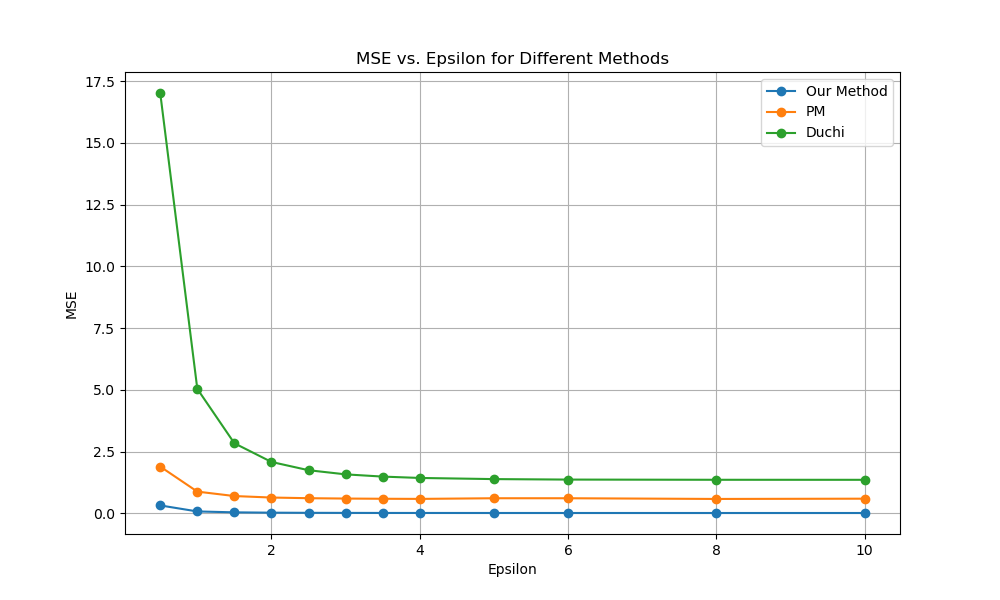
\includegraphics[width=0.9\textwidth]{figs/evaluation_eps_mse.png}
  \caption{مقایسه‌ی میانگین مربعات خطای روش پیشنهادی با دو روش پی.اِم و دوچی}
  \label{fig:eps_mse}
\end{figure}

همچنین نمودار \رجوع{fig:eps_avg}، میانگین اختلاف توزیع احتمال را برای سه روش مختلف و در سطوح بودجه‌ی حریم خصوصی، به تصویر می‌کشد. معیار میانگین اختلاف توزیع احتمال نشان می‌دهد که توزیع داده‌های نوفه‌دار شده تا چه حد به توزیع داده‌های اصلی شباهت دارد و مقدار کمتر آن، به معنای عملکرد بهتر است.

روش پیشنهادی (خط آبی)، پایداری مطلوبی داشته و در تقریباً تمام بازه $\epsilon$، کمترین میزان اختلاف را با توزیع اصلی داده‌ها نشان می‌دهد. این موضوع حاکی از توانایی بالای این روش در حفظ ساختار آماری و ویژگی‌های بنیادین داده‌هاست. در مقابل، روش دوچی (خط سبز) نه تنها در اکثر محدوده‌ها بیشترین میزان اختلاف را دارد، بلکه در مقادیر پایین $\epsilon$ رفتاری نامنظم و غیریکنواخت از خود بروز می‌دهد. این نوسان شدید، که احتمالاً ناشی از ماهیت تصادفی برخی عملیات‌های به کار رفته در این الگوریتم است، قابلیت اطمینان آن را کاهش می‌دهد. روش پی.اِم اگرچه از روش دوچی بهتر عمل می‌کند، اما همچنان با اختلاف قابل توجهی ضعیف‌تر از روش پیشنهادی ظاهر شده است. در نتیجه، می‌توان گفت الگوریتم ارائه شده در شرایطی که بودجه‌ی حریم خصوصی محدودی داریم، راهکاری بسیار دقیق‌تر و پایدارتر برای حفظ توزیع اصلی داده‌ها است.

\begin{figure}[h]
  \centering
  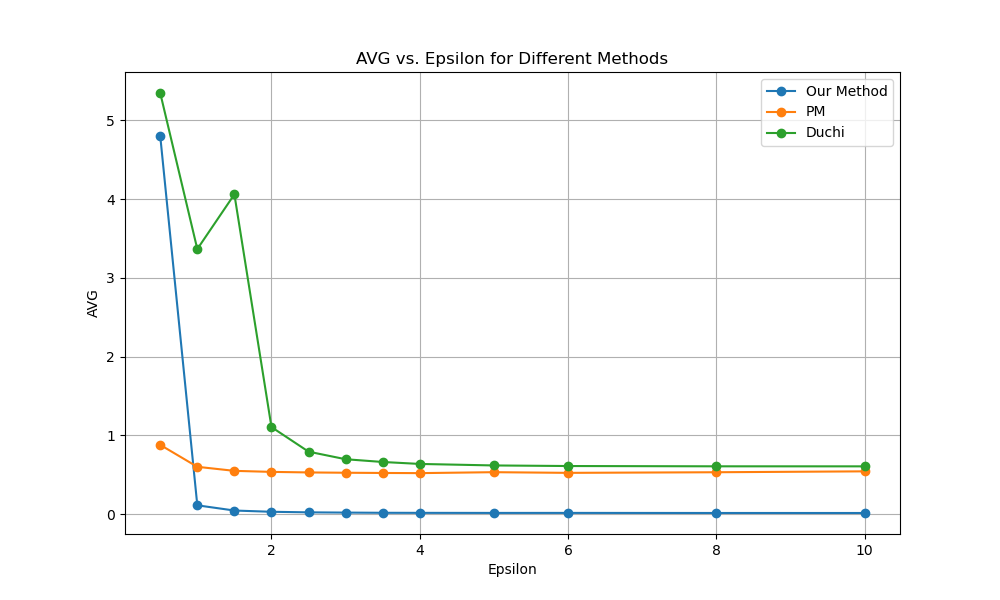
\includegraphics[width=0.9\textwidth]{figs/evaluation_eps_avg.png}
  \caption{مقایسه‌ی میانگین اختلاف توزیع احتمال داده‌ها در روش پیشنهادی با دو روش پی.اِم و دوچی}
  \label{fig:eps_avg}
\end{figure}

\زیرقسمت{ارزیابی حین تغییر تعداد ابعاد داده}

نمودار \رجوع{fig:dim_avg}، عملکرد سه روش مختلف را در مواجهه با افزایش تعداد ابعاد داده‌ها ارزیابی می‌کند. محور افقی نشان‌دهنده تعداد ابعاد و محور عمودی، میانگین خطای هر روش است. در تحلیل داده‌های پیچیده، پایداری یک الگوریتم در برابر افزایش ابعاد، یک شاخص کلیدی برای سنجش کارایی آن محسوب می‌شود.

روش پیشنهادی (خط آبی) برتری مطلق خود را به نمایش می‌گذارد. این روش در تمام طول بازه، با حفظ میانگین خطا در سطحی بسیار پایین و نزدیک به صفر، عملکردی بسیار پایدار از خود نشان می‌دهد. این ثبات، یک مزیت کلیدی است، زیرا نشان می‌دهد که با پیچیده‌تر شدن داده‌ها و افزایش ابعاد، کارایی الگوریتم کاهش پیدا نمی‌کند. روش پی.اِم (خط نارنجی) اگرچه از پایداری نسبی برخوردار است، اما سطح خطای آن به مراتب بالاتر از روش ما باقی می‌ماند. در مقابل، روش دوچی (خط سبز) نه تنها با اختلاف زیادی بیشترین خطا را دارد، بلکه با افزایش ابعاد، رفتاری نامنظم و غیرقابل پیش‌بینی از خود نشان می‌دهد. این نوسانات شدید بیانگر آن است که این روش به شدت به تغییرات در تعداد ابعاد حساس است و قابلیت اطمینان پایینی دارد.

\begin{figure}[h]
  \centering
  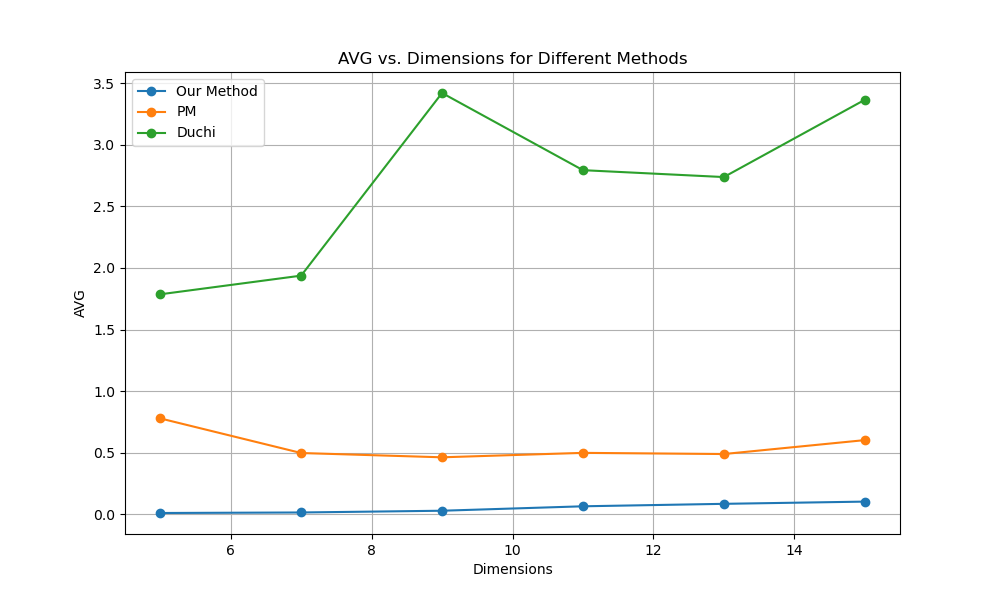
\includegraphics[width=0.9\textwidth]{figs/evaluation_dim_avg.png}
  \caption{مقایسه‌ی خطا در روش پیشنهادی حین تغییر تعداد ابعاد با دو روش پی.اِم و دوچی}
  \label{fig:dim_avg}
\end{figure}

\زیرقسمت{ارزیابی روی مجموعه داده‌های مختلف}

نمودار \رجوع{fig:dst_mse}، به ارزیابی عملکرد و قابلیت تعمیم‌پذیری سه روش مختلف در مواجهه با مجموعه داده‌های گوناگون می‌پردازد. روی محور افقی، برای هر مجموعه داده‌ی ورودی یک عدد تخصیص داده شده است و محور عمودی، میانگین مربعات خطا را نشان می‌دهد که مقدار کمتر آن، نشان‌دهنده دقت بالاتر است. بعضی از مجموعه داده‌ها نیز شامل مقادیر دودویی هستند.

روش پیشنهادی به‌طور پیوسته، کمترین میزان خطا را در تمامی مجموعه داده‌ها به ثبت رسانده است. این پایداری و دقت بالا نشان می‌دهد که الگوریتم ما از قابلیت تعمیم‌پذیری بسیار خوبی برخوردار است و عملکرد آن وابسته به نوع خاصی از توزیع داده نیست. در برخی نقاط، روند تغییرات خطا در روش پیشنهادی و روش پی.اِم شباهت‌هایی دارد؛ برای مثال، بین مجموعه‌ داده‌های شماره ۱۰ تا ۱۱، هر دو روش شاهد کاهش خطا بوده‌اند. این شباهت عملکرد در نمودار \رجوع{fig:dst_avg} که خطای احتمال توزیع مشرک داده‌ها را می‌سنجد، بیشتر به چشم می‌خورد.

\begin{figure}[h]
  \centering
  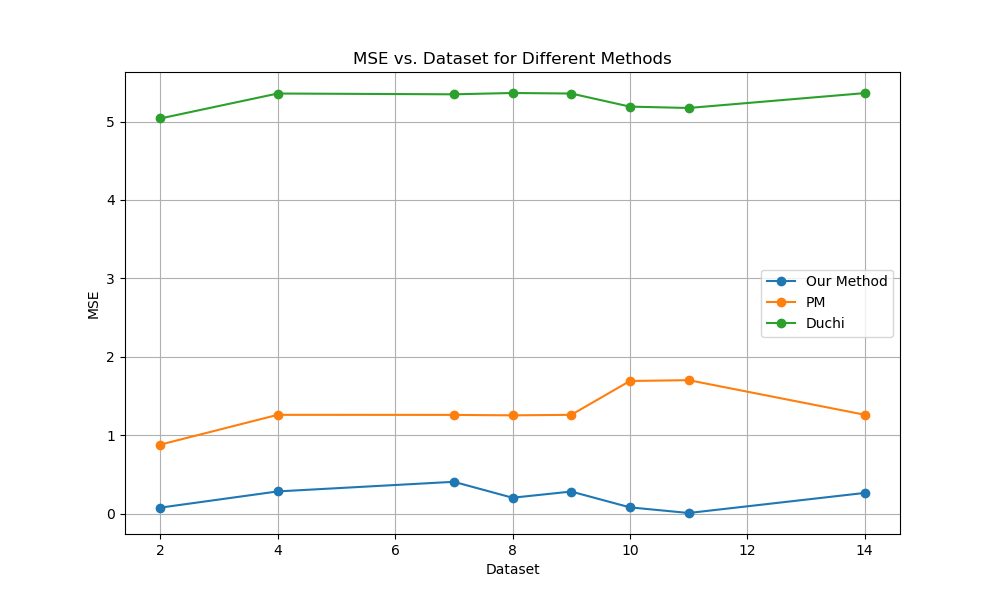
\includegraphics[width=0.9\textwidth]{figs/evaluation_dst_mse.png}
  \caption{مقایسه‌ی میانگین مربعات خطا در روش پیشنهادی حین تغییر مجموعه داده ورودی}
  \label{fig:dst_mse}
\end{figure}

\vspace{5pt}

\begin{figure}[h]
  \centering
  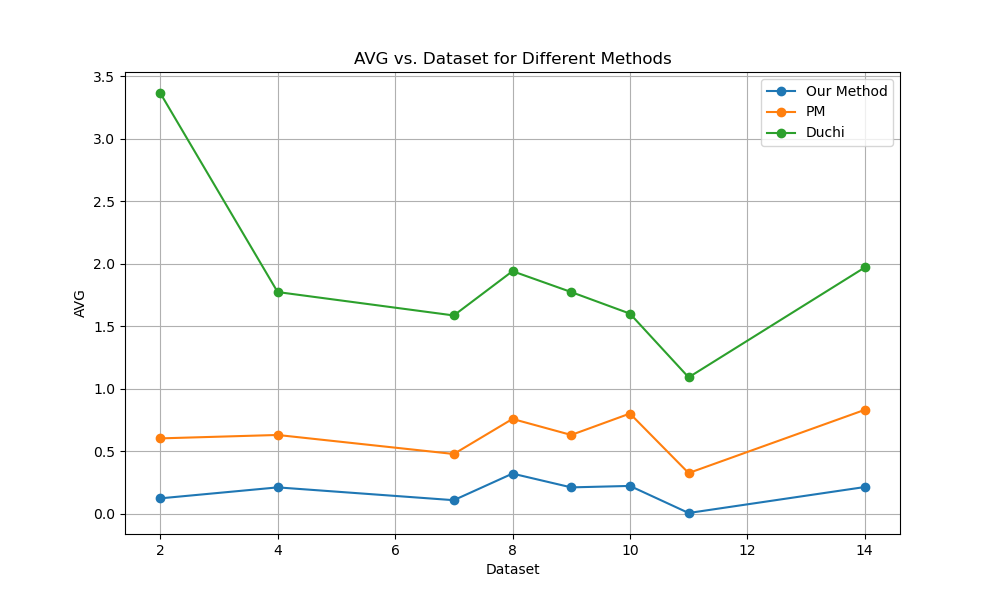
\includegraphics[width=0.9\textwidth]{figs/evaluation_dst_avg.png}
  \caption{مقایسه‌ی میانگین اختلاف توزیع احتمال داده‌ها حین تغییر مجموعه داده ورودی}
  \label{fig:dst_avg}
\end{figure}

\قسمت{ارزیابی روی داده‌های در حال تغییر}

محور عمودی نمودار \رجوع{fig:eps_frq} میانگین خطای تخمین شمارش را نشان داده و محور افقی نمایانگر تغییر بودجه‌ی حریم خصوصی است. الگوریتم پیشنهادی از نظر دقت، در سطحی کاملاً رقابتی و با فاصله‌ای ناچیز از دو روش رپور و دی.بیت.فلیپ.پی.اِم قرار دارد. در واقع بهبودهایی که روی حفظ حریم خصوصی داده‌های با ابعاد بالا انجام شده است، کمی دقت و سودمندی را کاهش داده است.

\begin{figure}[h]
  \centering
  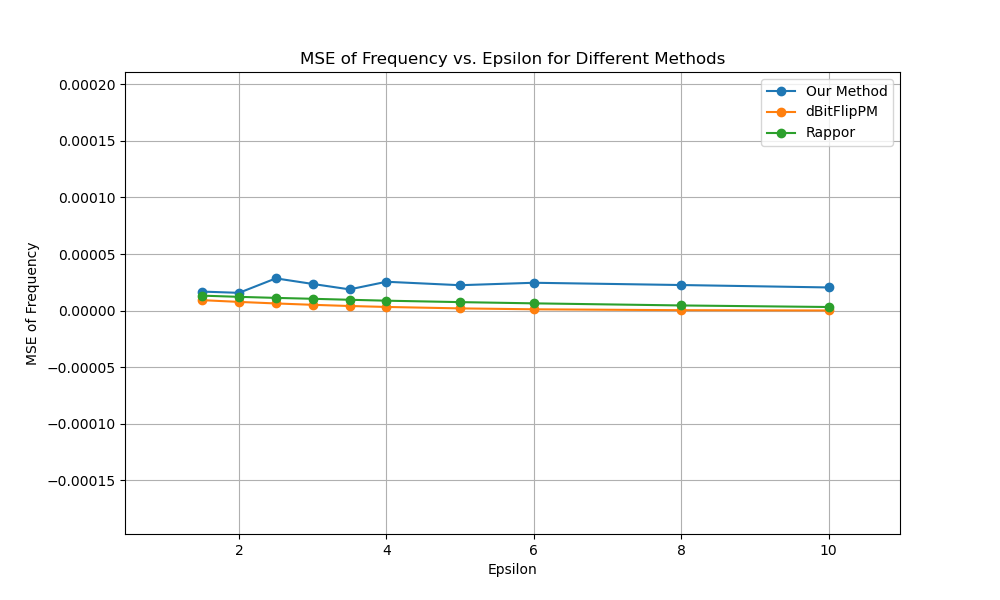
\includegraphics[width=0.9\textwidth]{figs/evaluation_eps_frq.png}
  \caption{مقایسه‌ی میانگین خطای تخمین شمارش در روش پیشنهادی حین تغییر بودجه‌ی حریم خصوصی}
  \label{fig:eps_frq}
\end{figure}

البته همانطور که در نموارد \رجوع{fig:usr_tim} مشاهده می‌کنید، با افزایش تعداد کاربران، زمان اجرای الگوریتم دی.بیت.فلیپ.پی.ام به صورت قابل توجهی افزایش می‌یابد. در مقابل، روش پیشنهادی با یک شیب بسیار ملایم‌تر، بهینگی مطلوبی را در مقیاس‌های بزرگ به نمایش می‌گذارد. این برتری در زمان اجرا، الگوریتم ما را به گزینه‌ای بسیار کارآمدتر برای پیاده‌سازی در سیستم‌های واقعی با میلیون‌ها کاربر تبدیل می‌کند. این مورد هم باید در نظر گرفت که الگوریتم رپور، با وجود خطای کمتر و سرعت بیشتر، دارای یک ضعف ذاتی در مواجهه با داده‌های در حال تغییر است. همانطور که قبل‌تر گفته شد، رپور در مواجه با داده‌هایی که به صورت مکرر تغییر می‌کنند ضعف داشته و به ازای هر تغییر کوچک، باید مقدار جدیدی حفظ کند. این فرایند روش حفظ کردن را زیر سوال برده و باعث نقض حریم خصوصی می‌شود. الگوریتم پیشنهادی این چالش کلیدی را به طور مستقیم هدف قرار داده و با ارائه‌ی یک سازوکار مقاوم، تضمین می‌کند که حریم خصوصی تفاضلی محلی حتی در صورت تغییر مداوم داده‌ها نیز به قوت خود باقی بماند.

\begin{figure}[h]
  \centering
  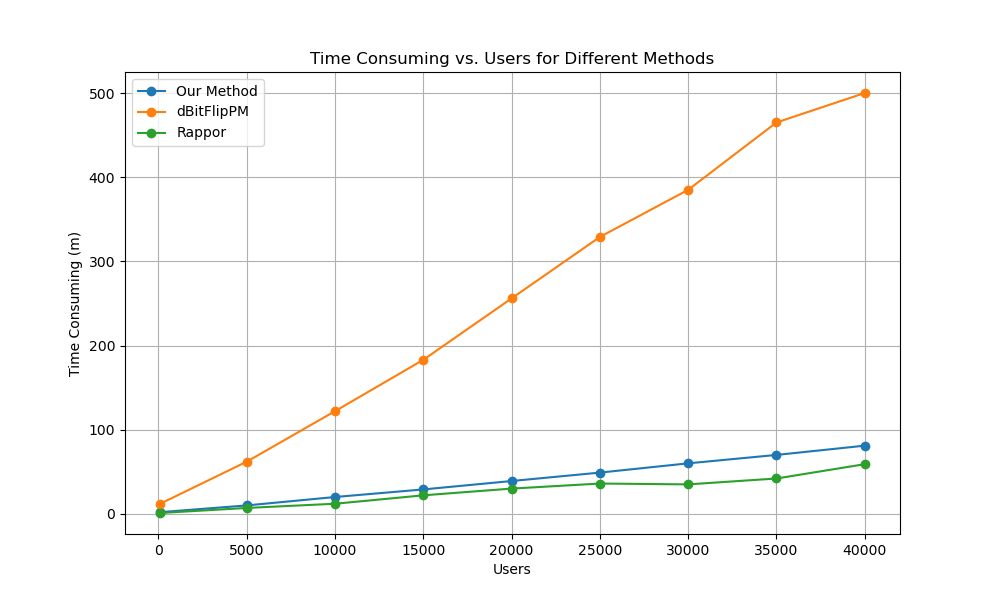
\includegraphics[width=0.9\textwidth]{figs/evaluation_usr_tim.png}
  \caption{مقایسه‌ی زمان اجرای الگورتیم پیشنهادی با دو روش رپور و دی.بیت.فلیپ.پی.اِم}
  \label{fig:usr_tim}
\end{figure}



